\section{Experiments}
\label{sec:experiments}
This section discusses how the models are trained and selected, and how they are evaluated. Firstly, the conventional measures and the Gemini-based metrics are computed on the same outputs to see whether they agree \textbf{(RQ1)}. Secondly, fine-tuning runs are trained where each run weights one kind of error more heavily, to demonstrate how the leaked and invented errors interact \textbf{(RQ2)}. Finally, the baseline and the extension are compared on Gemini's errors, how often the right voice is picked and the delay, to show what the voice information adds in real time \textbf{(RQ3)}.


  \subsection{Training setup}
  \label{sec:training}
  The training setup is described below and considers how the training data is augmented, the optimisation and hardware used, how the final model is selected, the systems compared, and the actual training observed.
  \subsubsection{Data augmentation}
  \label{exp:augmentation}
  The training data is augmented with varying strategies to prevent overfitting. The first strategy is to provide every trial twice per epoch where the target and interferer roles are swapped. This means the same mixture requires two different outputs where the only varying information is the enrollment clip. If a clip is only used once for a single speaker, the answer remains the same which can be memorised. Therefore the swap ensures that if the model memorises on one voice, it will be penalised if it fails to generalise to the other voice. The second strategy is to rotate enrollment clips for a target speaker. Each speaker per trial rotates between 3 enrollment clips so that the model does not memorise a single enrollment to a speaker. The third strategy is to randomly perturb the noise and reverberation for each trial per epoch. Finally, in the spirit of stochastic methods, a single random \SI{4}{\second} crop is taken from a random position in the trial for each epoch.

  \subsubsection{Optimisation and hardware}
  \label{exp:hyperparam}
  % AdamW, learning rate, weight decay, gradient clip, batch 3, mixed precision, LR halving, early stopping, silence warm-up, seed 42, Tesla T4
  During training the AdamW optimiser \cite{loshchilov2019adamw} was used with a base learning rate of \num{0.0005}, weight decay of \num{0.0001} and gradient clipping at \num{5.0}. A batch size of 3 was used, thus 6 samples were processed per iteration (see \autoref{exp:augmentation}) with mixed precision training. The learning rate schedule included halving the learning rate when the Whisper WER stops improving. The target-absent term in the loss, $L_{\text{abs}}$, is off for the first 2 epochs, as the model in the early epochs would just output silence as this term is easy to optimise. The model is trained on Kaggle's Tesla T4 GPU for 12 hours per session and the random seed is set to 42 for reproducibility. 
 

  \subsubsection{Model selection}
    Training length was set by the 12-hour limit of a Kaggle GPU session rather than by the loss. An early stopping mechanism after 10 epochs without improvement was available as a backstop but never triggered. The baseline ran for one session of 14 epochs. The extension ran for 14 epochs, and because its in-training word error rate was still falling at the end of that session (its best epoch was the last), training was resumed for a second session, to 28 epochs.

  The final model to base the evaluation on cannot simply be chosen by the model with the lowest validation loss as a result of the proxy training objective. The loss (\autoref{sec:objective}) is a proxy for the downstream task, where the approach in the proxy is to reward better separation. However, better separation does not guarantee better recognition (\autoref{sec:evaluation}): the epoch with the lowest loss for the extension has the highest LCF-WER of the chosen checkpoints as seen in \autoref{fig:training_curves}. Secondly, the model cannot be optimised directly against the LCF-WER as it is not differentiable. Finally a consideration is that the live judge is also too slow to run after every epoch. The model is thus chosen as follows: Whisper (\autoref{sec:offline_asr}) during training will create a shortlist of best candidate checkpoints based on the WER of the validation set. The candidates are then scored by the live judge (\autoref{sec:live_judge}) on the validation set, where the lowest WER is chosen as the final model with ties broken by fewer invented words. 

  \subsubsection{Systems compared}
  \label{exp:systems}
  % Define the five once: No processing, Baseline, Extension, WeSep, Target alone (perfect).
    This work evaluates 3 models against the floor and ceiling (\autoref{sec:anchors}): baseline BSRNN (implemented following REAL-TSE \cite{wang2026realtse}; Section~\ref{sec:architecture}), the extension BSRNN with speaker context embedding (Section~\ref{sec:e_architecture}), and WeSep \cite{wang2024wesep}. There are four main reasons to include WeSep for comparison: \textit{(i)} the REAL-TSE challenge \cite{wang2026realtse}, which this work uses as a guideline, builds its baseline system with WeSep; \textit{(ii)} the WeSep model has the same BSRNN backbone with TF-Map cue of \cite{zhang2025multi} as this work's baseline and extension, where the main architectural difference is WeSep's use of contextual embeddings rather than the single embedding per enrollment clip used by the extension, as discussed in Section~\ref{sec:speaker_context_embedding}; \textit{(iii)} WeSep is used to validate the dataset constructed in this work, as WeSep was trained on clean Libri2Mix \cite{cosentino2020librimix} and thus has not heard any of the speakers in the evaluation sets, so its extraction demonstrates what an established model can recover from these mixtures; and \textit{(iv)} WeSep provides a stronger offline reference for extracting the target. The WeSep model itself is non-causal and almost four times the size of the baseline (27.2\,M versus 7.19\,M parameters), and thus shows what extraction can achieve when latency and model size are not a concern.

  WeSep was not trained on data that contained noise or reverberation, whereas trials in this work contain both. Secondly, WeSep itself has a causal separator; however, the features are normalised over the entire clip before the separator. This setup means that every output frame depends on audio that has not arrived yet and thus the model cannot be streamed and is treated as an offline system. Finally, the results of WeSep are not comparable to the results found in the REAL-TSE challenge \cite{wang2026realtse} due to varying data, metrics and protocols. 

 
  \subsubsection{Training curves}
  \label{exp:curves}
  Both models were trained with the same loss and the same settings, but differ in how long they were trained. The baseline was trained for 14 epochs and the extension for 28. \autoref{fig:training_curves} shows how the validation scores of each model changed during training. The top row of \autoref{fig:training_curves} shows the breakdown of the loss for the target-present branch. The three terms of the loss, shown separately, highlight how the terms interact with each other. A typical trend seen for both baseline and extension is that as the separation term $L_{\text{pres}}$ for training decreases (rather sharply), the validation separation very gradually decreases, and then very gradually increases again. A positive note to be seen is how the multi-resolution spectrum term, $L_{\text{MR}}$, consistently decreases for both training and validation, showing how the extractor is able to reconstruct the audio with fewer artefacts. The gain term for ensuring that the model produces audio at a similar level to the target, $L_{\text{gain}}$, follows the same trend as the separation term, which is slight decrease followed by a slight increase. Finally, the baseline model is only trained for one session, as by the validation live judge results it can be seen that on the final epoch the validation WER has reverted back to a same score as the fourth epoch. Epoch 11 is chosen for the baseline as it has the lowest validation WER. Although separation is not the hallmark indicator of a good extractor for the context of the downstream task, when the term is decreasing in conjunction with the spectrum term, it is a good indication to continue training. The extension model is thus trained for a second session as by the end of the first session, \textit{(i)} the Whisper WER is generally decreasing although sporadic, and \textit{(ii)} the separation term with the spectrum term is decreasing. Epoch 21 has a similar validation WER to epoch 27 (39.59\,\% against 39.23\,\%), and is preferred when considering the breakdown of the validation scores which is found in \autoref{app:epoch_choice}. Epoch 27 in 95--97\,\% of resampled validation sets causes Gemini to invent more words per trial (2.56 against 2.20) and to invent two or more words more often (55.5\,\% against 46.9\,\%) than epoch 21. The tradeoff is that epoch 27 almost always leaks less interfering speech in a trial (20.2\,\% against 23.1\,\%). Since the difference between the leftover speech and introduced artefacts is equally as strong (since the WER is similar) in this validation set, the choice is made to prioritise less invention as this will translate to more unseen trials. Leakage is target and interferer dependent, but artefacts will be produced whenever the model is used. Live models struggle more with extractor artefacts than with leftover noise (\autoref{sec:evaluation}, \cite{iwamoto2022bad}), thus the epoch with fewer artefacts is preferred. 
  % Training curves, baseline (matched protocol) and extension on shared axes. Drawn for this work by
%   ../tse_venv/bin/python scripts/plot_training_curves.py --layout terms-wer --out report/figures/training_curves.pdf
% from both runs' history.csv and every matching live-judge run
% (sir0_val, both, n=103). Baseline = 2026-10-07-train-sir0-baseline-matched-s1, session 1
% of 2 (epochs 0-13); session 2 and its judge runs appear on re-running the command above
% once they exist. The original 16-epoch baseline run (2026-09-04) is no longer drawn.
\begin{figure}[htbp]
  \centering
  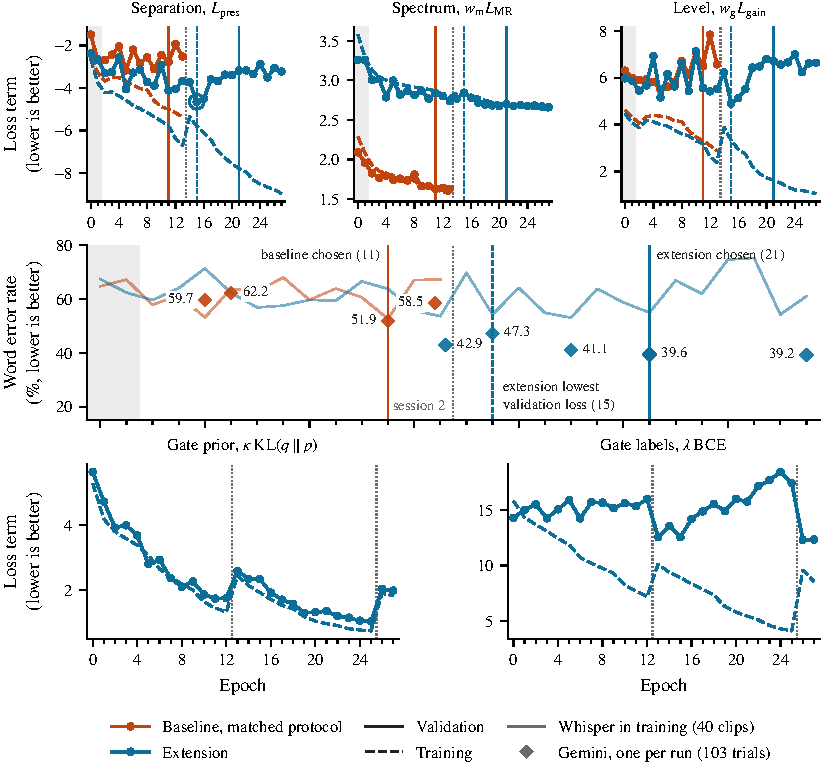
\includegraphics[width=\textwidth]{figures/training_curves.pdf}
  \caption{The baseline (orange) and the extension (blue), trained under the same protocol. The top row shows the three weighted terms of the target-present loss which are attributed to target specific components, as seen in the first bracket of \autoref{eq:total}. The middle row shows the word error rate on the 103 validation trials with both speakers present. Each diamond is one run of the live judge on the same audio. The solid vertical line marks the chosen epochs, and the grey dotted line where training resumed in a second session. The bottom row shows the loss curve of the presence gate, which is only trained on the extension. }
  \label{fig:training_curves}
\end{figure}

  
  


 \subsection{Evaluation setup}
 The evaluation setup is described below and considers the listeners used, the latency measures, and the evaluation metrics. The evaluation metrics are described in \autoref{sec:metrics} and the results of the evaluation are presented in \autoref{sec:results}.
  \subsubsection{Listeners}
  \label{sec:transcription}

  \paragraph{Offline ASR model}
  \label{sec:offline_asr}
  The offline transcriber is the \texttt{faster-whisper} implementation \cite{faster_whisper} of the Whisper \cite{radford2023whisper} model, run with the \texttt{large-v3-turbo} checkpoint. This is Whisper large-v3 with its decoder pruned from 32 layers to 4 and then fine-tuned, giving 809\,M parameters against the 1{,}550\,M of large-v3 \cite{whisper_turbo}. The large Whisper variants are a common choice for scoring how intelligible generated and extracted speech is \cite{anastassiou2024seedtts,wang2025solospeech}. Decoding was greedy, with a single sampling temperature of zero and no conditioning on previously decoded text, so the same audio always produces the same transcript, and the language was fixed to English. The smaller \texttt{small.en} checkpoint (244\,M parameters) is used only inside the training loop, where it transcribes a validation sample every epoch to shortlist checkpoints and schedule the learning rate. 


  \paragraph{Live judge}
  \label{sec:live_judge}
  The live listener is \texttt{gemini-3.7-flash} \cite{google2026geminilive}, which was connected to via the \texttt{google-genai} Python package through the Application Programming Interface (API). The judge, like the ASR model, does not separate anything. The Gemini model is prompted to transcribe what it can hear in the extractor's output. The live model is the tool for which this work is being built and so its result is the most important with respect to the overall evaluation of the extractor. 

  The prompt used can be found in \autoref{app:prompt}. It is deliberately worded to avoid instructing the judge to pick a speaker to prevent the judge acting on the extractor's behalf. Secondly, it does not instruct the judge to guess as this would be a form of hallucination, which is a metric that is being measured and thus should not be confounded by the prompt. Finally, since live models by default will return some kind of response, the judge is prompted to return a structured response of a status field alongside the transcript. The status field is used to indicate whether the judge heard speech or not, and if it did not hear speech, the transcript is left empty. This allows for a clear distinction for whether the model hallucinates as the status field can be used to determine whether the model heard speech or not.

  \paragraph{Speech gating}
  \label{sec:speech_gate}
The Silero VAD v6.2.1 \cite{silero2021vad} speech gate is implemented to filter out any audio that appears to contain no speech; it acts as a pre-filter for the transcription tools. This method was considered for four reasons: \textit{(i)} if the gate is applied to a mixture that contained speech and the gate determines that the estimated audio does not contain speech, then it is already an indication that the extractor has failed to extract the target speaker, \textit{(ii)} if the gate is applied to a mixture that does not contain speech and the gate determines that the estimated audio does contain speech, then it is already an indication that the extractor has hallucinated, \textit{(iii)} if the gate is applied to a mixture that does not contain speech and the gate determines that the estimated audio does not contain speech, then it is already an indication that the extractor has correctly determined that there is no speech, and \textit{(iv)} this method is a practical implementation in a real system thus has a natural application to the evaluation of the extractor. Therefore it covers all possible scenarios and is a practical solution to the problem of hallucination. This method is supported by \cite{whisper_hallucination_2025} and is applied for both the ASR and live judge.
  

  \subsubsection{Latency measures}
 The latency of the different systems was measured to compare the implemented model against \textit{(i)} the latency specification for live transcription, and \textit{(ii)} the latency of established systems. There are two components to consider: time to consume and time to process the audio. The first component considers the real-time factor (RTF). The RTF is the ratio of the time taken to process the audio to the length of the audio, and for a model to be able to keep up with real-time audio, the RTF must be less than 1. The second component considers the latency created by the architecture itself which cannot be improved by faster hardware. To produce the output frame for a given window, the model must first have received that entire window. This forces a delay of the processing of the window as per \autoref{sec:stft}. 

 A real-time factor alone cannot distinguish a model that is merely slow from one that requires the entire utterance. An implemented probe replaces all audio after a time $T$ and measures how far the output \emph{before} $T$ moves: if changing the future changes what the model has already produced, then that output depends on audio which has not yet arrived, and the model cannot be streamed. For a strictly causal model the movement must be zero. The replacement is made at matched loudness so that the overall level of the input is preserved.

